\documentclass{article}
\usepackage[a4paper, margin=1in]{geometry} % Adjust margin size as needed
\usepackage{graphicx} % Required for inserting images
\usepackage{listings}
\lstset{basicstyle=\ttfamily}
\usepackage{float}
\usepackage{courier}
\usepackage{tabularx}
\usepackage{tikz}
\usepackage{url}
\usepackage{amsmath}
\usepackage{float}
\usepackage{hyperref}
\usepackage{MnSymbol}
\usepackage{indentfirst}

\title{Project: Report Document}
\author{Daniel Alejandro Marin - R11858881\\ \\ Texas Tech University \\CS3375 - Computer Architecture \\ Instructor: Dr. Juan Carlos Rojas}
\date{December 6$^{th}$, 2024}
\begin{document}
\maketitle
\tableofcontents
\newpage
\section{Introduction}
Instruction scheduling plays a crucial role in moder computer architecture, especially for achieving high performance in multi-issue processors; they allow for faster instruction throughput. This project aims to simulate the shceduling of `assembly' instructions under various processor configurations. The configurations developed in this project are the following:
\begin{itemize}
    \item Single-issue Instruction Scheduler (in-order)
    \item Superscalar Instruction Scheduler (in-order)
    \item Superscalar Instruction Scheduler (out of order) 
\end{itemize}

\indent For each of this configurations there exists a version with register renaming and one without. In this project, we will simulate a the scheduling of a simple assembly instruction set, in each of these configurations.
\newline
\indent Throughout this report document, we will be explaining the design, implementation details, test and results of each configuration. The insights gained will highlight the advantages and limitations of these techniques in processor architectures. 
\section{Design}
The instruction scheduling simulation system is designed as a hierarchy of classes that simulate different types of processor configurations for instruction fetching and retirement. The design uses abstraction and inheritance to encapsulate common functionality while allowing customization for specific scheduling techniques like: register renaming, in-order retirement, etc\ldots Following is a class diagram that encapsulates the core design of this project:
\begin{figure}[H]
    \centering
    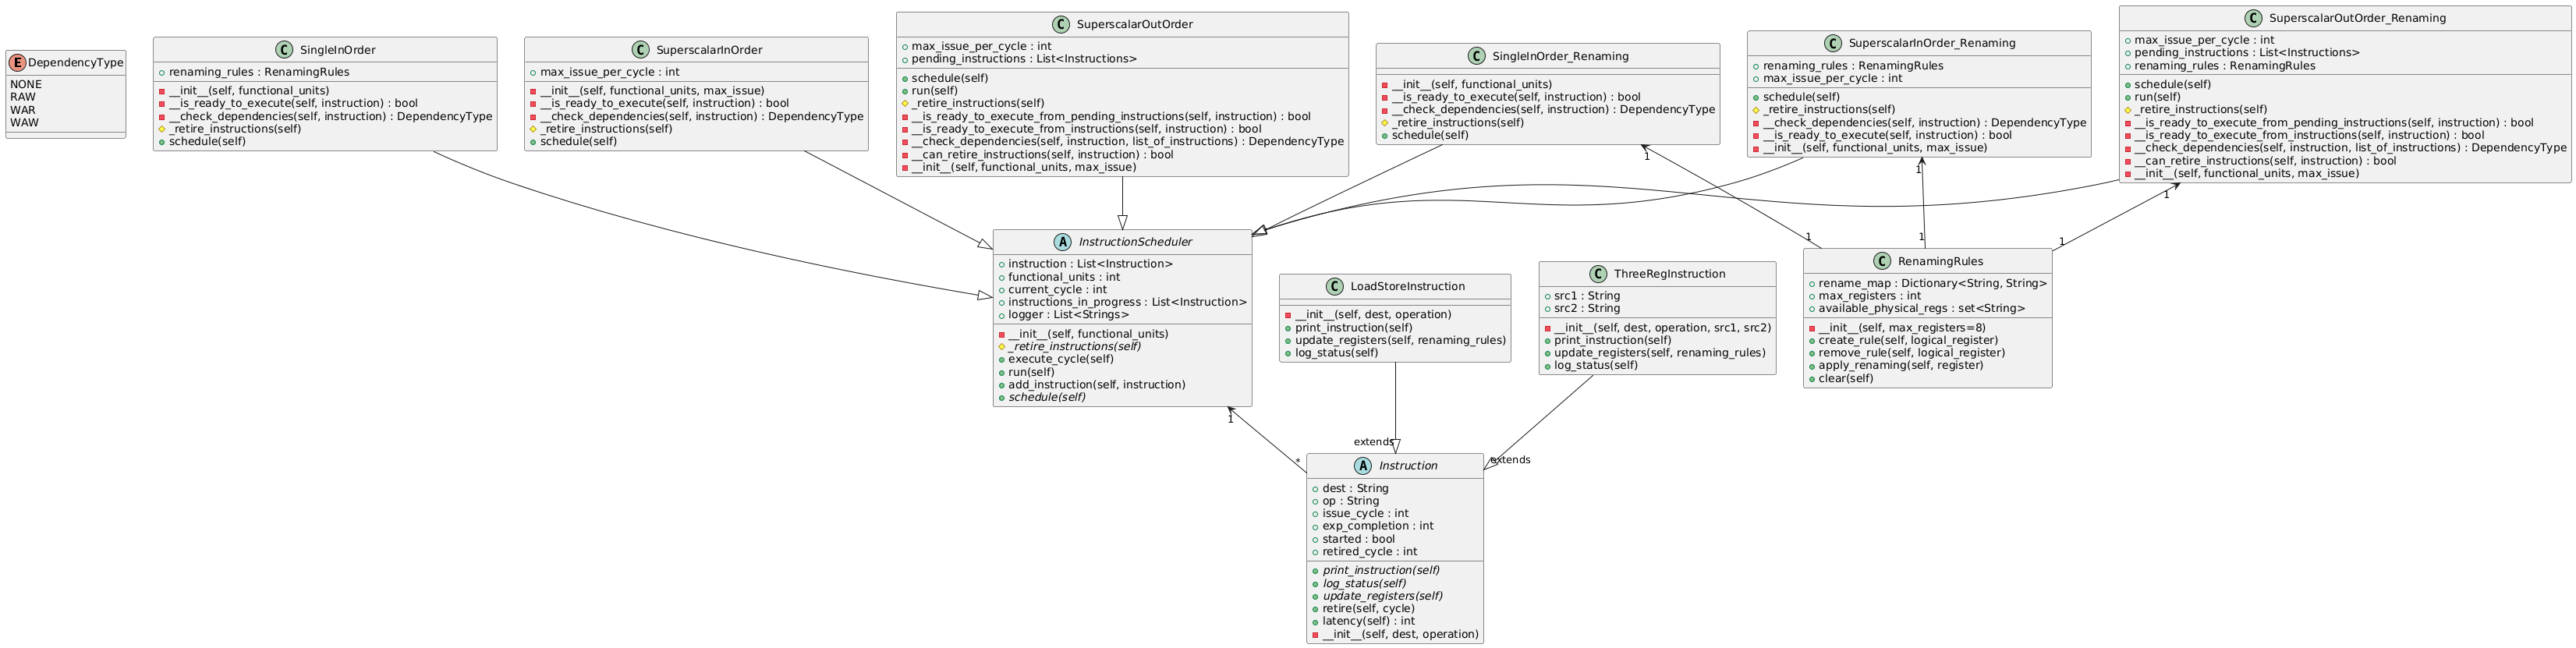
\includegraphics[width=1\textwidth]{ClassDiagram.png}  
    \caption{Class Diagram of Design, developed using the Plant UML tools.}  
    \label{fig:ClassDiagram}
\end{figure}
The diagram in figure \ref{fig:ClassDiagram} encapsulates the logic that helped develop this simulation. In the following subsections, I will be explaining the logic and reasons behind each class seen in here.

\subsection{Instruction Scheduler Abstract Class}
The \lstinline|InstructionScheduler| abstract class defined the layout all configurations of instructions schedulers should follow. It defined the main components and methods they should have, and contained some of the overlapping logic that remained consistent throughout all configurations. It contained the following properties:
\begin{itemize}
    \item \lstinline|instructions|: this property looks to contain a list of instructions that need to be scheduled in the simulation.
    \item \lstinline|functional_units|: this property represents the number of parallel functional units the scheduler has. It is a property defined by the user. 
    \item \lstinline|current_cycle|: this property contains the current cycle of execution of the processor.
    \item \lstinline|instructions_in_progress|: this property contains the list of instructions that are currently being executed. 
    \item \lstinline|logger|: this property contains a `log book' of the logs performed by the scheduler, used for debug statements and keeping track of instructions in the order they retire (outputs).
\end{itemize}

These are the properties all schedulers contained, additional properties can be added to the subclasses of \lstinline|InstructionScheduler| when needed. Now, let's look at the methods defined in this parent class in the following itemize:
\begin{itemize}
    \item \lstinline|__init__(self, functional_units=1)|: this constructor method is used to create instances of this class, and it is called by the children classes as to initialize the aforementioned properties. 
    \item \lstinline|add_instruction(self, instruction)|: this method is in charge of adding an instruction to \lstinline|instructions|. It is used to add parsed instructions set that we want to simulate the scheduling.
    \item \lstinline|execute_cycle(self)|: this method contains the logic of executing a cycle in the simulation incrementing \lstinline|current_cycle| by one, attempting to schedule instructions, and retiring instructions. The definition is as follows:
    \begin{lstlisting}
    def execute_cycle(self):
        self.current_cycle += 1
        self.schedule()
        self._retire_instructions()
    \end{lstlisting}
    \item \lstinline|run(self)|: this method is fairly straightforward, it executes cycles until all instructions have been dispatched out of the scheduler. Most configurations used the definition:
    \begin{lstlisting}{language=Python}
    def run(self):
        while self.instructions or self.instructions_in_progress:
            self.execute_cycle()
    \end{lstlisting}
    \item \lstinline|schedule(self)|: this method contains the logic for scheduling instructions. It is abstract, since each subclass configuration schedules instructions differently. 
    \item \lstinline|_schedule_instruction(self, instr : Instruction)|: this method is in charge of updating the status of an instruction whenever it gets scheduled. It does so in the following manner:
    \begin{lstlisting}{language=Python}
    def _schedule_instruction(self, instr : Instruction):
        instr.issue_cycle = self.current_cycle
        instr.exp_completion = self.current_cycle + instr.latency()
        instr.started = True 
        self.instructions_in_progress.append(instr)
    \end{lstlisting}
    \item \lstinline{_retire_instructions(self)}: this method should contains the logic for retiring instructions. It is abstract, since each subclass configuration retires instructions differently.
\end{itemize}


\section{Methodology}

\section{Tests}

\section{Results}

\section{Discussion}

\end{document}